\documentclass[11pt]{article}
%you can look for fun LaTeX packages to use hereasdf

\usepackage{amsmath}
\usepackage{amssymb}
\usepackage{fancyhdr}
\usepackage{amsthm}

\usepackage{graphicx}
\usepackage{dcolumn}
\usepackage{bm}

%fun commands for fun sets
%make sure to use these in math mode
\newcommand{\Z}{\mathbb{Z}}
\newcommand{\R}{\mathbb{R}}
\newcommand{\N}{\mathbb{N}}
\newcommand{\C}{\mathbb{C}}
\newcommand{\m}{\mathcal{M}}
\newcommand{\Tt}{\mathcal{T}}
\newcommand{\pa}{\partial}
\newcommand{\dD}{\mathcal{D}}
\newcommand{\E}{\mathbb{E}}



\oddsidemargin0cm
\topmargin-2cm    
\textwidth16.5cm   
\textheight23.5cm  

\newcommand{\question}[2] {\vspace{.25in} \hrule\vspace{0.5em}
\noindent{\bf #1: #2} \vspace{0.5em}
\hrule \vspace{.10in}}
\renewcommand{\part}[1] {\vspace{.10in} {\bf (#1)}}

\newcommand{\myname}{Alex Havrilla}
\newcommand{\myandrew}{alumhavr}
\newcommand{\myhwnum}{Hw 1}

\newtheorem{theorem}{Theorem}
\newtheorem{prop}{Prop}
\theoremstyle{remark}
\newtheorem{lemma}{Lemma}
\newtheorem{remark}{Remark}
\newtheorem{defi}{Def}
\newtheorem{apps}{Application}
\newtheorem{quest}{Question}
\newtheorem{ans}{Answer}
\newtheorem{interest}{Interesting}
\newtheorem{theme}{Theme}
\newtheorem{back}{Background}
\newtheorem{idea}{Idea}
\newtheorem{example}{Example}

\setlength{\parindent}{0pt}
\setlength{\parskip}{5pt plus 1pt}
 
\pagestyle{fancyplain}
\lhead{\fancyplain{}{\textbf{HW\myhwnum}}}      % Note the different brackets!
\rhead{\fancyplain{}{\myname\\ \myandrew}}
\chead{\fancyplain{}{\mycourse}}

\linespread{1.3}

\title{Deadlines}

\begin{document}

\maketitle

\section{3/9}

\subsection{Goals}

\begin{enumerate}
	\item Work on thesis: finish 2 sections
	\item Work on complex: finish 2 problems
	\item Work on drl: finish 1 problem
\end{enumerate}

\subsection{DRL}

\begin{remark}
	Recall: Goal is to learn $v_{\pi}(s)$ from episodes of experiece under $\pi$.(In MC or TD learning)

	For Monte Carlo: Update $V(S_t) := V(S_t) + \alpha(G_t -V(S_t))$ over random trajectories
\end{remark}

\begin{remark}
	Monte-Carlo: $G_t$ is unbiased estimator of $V_{\pi}(S_t)$. But potentially high variance

	Temportal Difference: $R_{t+1}+\gamma V(S_{t+1})$ is biased estimator but lower variance. True target $R_{t+1} + \gamma v_{\pi}(S_{t+1})$ is unbiased estimate of $v_{\pi}(S_t)$
\end{remark}

\begin{remark}
	Note this is idea of bootstrapping: using data to generate model which we then use in estimator: estimator uses another estimator.
\end{remark}

\begin{remark}
	SARAS and q-learning method of updating q values
\end{remark}

\section{3/10}

\subsection{Goals}

\begin{enumerate}
	\item Finish complex/study
	\item Study DRL
	\item Read evolution
\end{enumerate}

\subsection{Complex Analysis}

\begin{quest}
	If f entire can we expand in powerseries converging everywhere?
\end{quest}

\subsection{DRL Review}

\begin{verbatim}
	https://cmudeeprl.github.io/403_website/assets/lectures/s21/s21_rec2_gaussian_process.pdf
\end{verbatim}

\begin{remark}Gaussian Process OPtimization: 
\begin{verbatim}
	C. E. Rasmussen & C. K. I. Williams, Gaussian Processes for Machine Learning, the MIT Press, 2006
\end{verbatim}
\end{remark}

\begin{remark}Kernel Cookbook:
\begin{verbatim}
	https://www.cs.toronto.edu/~duvenaud/cookbook/
\end{verbatim}
\end{remark}

\begin{remark}
	Example of learning continuous problem: ON some manifold: transition function is $T(s,a) = cos(sa)$ and reward function is $r(s,a) = -s^2$. 
\end{remark}

\begin{quest}
	Difference between $GP-CEM$ and regular CEM?
\end{quest}


\begin{remark}
	Limitations of GP:
	\begin{enumerate}
		\item Hard to approximate kernel in DRL
		\item COmputation complexity of inference hard $O(n^3)$ (matrix inversion)
		\item Hard to design differentiable policy/action optimization techniques
		\item Designing multi-variante GPs is hard
	\end{enumerate}
\end{remark}

\begin{remark}
	GP: Can fully represent epistemic uncertainty, but not allows practical. 
\end{remark}

\begin{remark}
	Limitations of learning by interaction:
	\begin{enumerate}
		\item needs chance to try and fail many times
		\item Hard when safety a concern
		\item hard inr eal life which takes time
	\end{enumerate}
\end{remark}

\begin{remark}
	Challenges in imitation learning:
	\begin{enumerate}
		\item Compounding errors
		\item Non-markovian observation
		\item Lack of generalization
	\end{enumerate}
\end{remark}

\begin{remark}
	Compunding errors happen when we make an error which causes us to deviate farther from expert which makes us more likely to make error at next time step. 

	Fix is to augment training with error cases so we can self correct when necessary
\end{remark}

\begin{remark}
	Can concatenate states to make markovian issues nonissues. Just redfine "state". Or use RNNs, which are inherently nonmarkovian, since they feed input as well as transformed input
\end{remark}

\begin{remark}
	There is always one optimal policy: $v_*(s) = max_{\pi}(\pi(s))$
\end{remark}

\begin{remark}
	Solving the MDP is finding the state and action value functions given a policy
\end{remark}

\begin{remark}
	Optimal value functions measure the best possible goodness of states or state/action pairs under all policies. So actually this is THE optimal policy vs. all others. 
\end{remark}

\begin{quest}
	If the optimal policy is simply the one which maximizes return at each state, what's the problem?
\end{quest}

\begin{quest}
	I guess the definition is recursive.
\end{quest}

\begin{remark}
	\begin{align*}
		\E[G_t | S_t = s] = \E[R_{t+1} + \gamma G_{t+1} | S_t = s]
	\end{align*}
	\begin{align*}
		v_{\pi}(s) = \E[R_{t+1} + \gamma v_{\pi}(S_{t+1})] = \sum_a \pi(a|s) \sum_{s',r}p(s',r|s,a)[r+\gamma v_{\pi}(s')]
	\end{align*}
\end{remark}

\begin{remark}
	Bellman expectation equations give us a S equations linear where S is number of states. Can be solved with linear system solver. $q^*$ unique solution to system of nonlinear equtions
\end{remark}

\begin{remark}
	MDP under fixed policy is MRP:

	$v_{\pi}(s) = r_s^{\pi}+\gamma \sum_{s' \in S}T_{s's}^{\pi}v_{\pi}(s')$

	where $r_s^{\pi} = \sum_{a \in A}\pi(a | s) r(s,a)$ and $T_{s's}^{\pi} = \sum_{a \in A}\pi(a|s)T(s'|s,a)$
\end{remark}

\begin{quest}
	What does it mean under fixed policy? I thought policy already given? Do we mean deterministic rewards? THis is mathematically plausible
\end{quest}

\begin{remark}
	$v_{\pi} = (I-\gamma T^{\pi})^{-1}r^{\pi}$ where we have a matrix over states $T^{\pi}$ which are transitions from one to the other. But matrix inversion costly 

	The advantage in fixing a policy is that we have a transition matrix(since we know what actions we'll take).
\end{remark}

\begin{remark}
	We know there is a unique optimal policy $\pi^*$ w.r.t total dominance partial ordering $\pi \geq \pi'$
\end{remark}

\section{3/11}

\subsection{Goals}

\subsection{Modeling Evolution}

\begin{remark}
	Stochastic Switching: phenotypic hetergeneity despite genotypic uniformity. A bet heding strategy when mutation isn't enough.
\end{remark}

\begin{quest}
	How is phenotypic configuration preserved if genotype uniform(from one generation to next). What else is passed on (methylation patterns?).
\end{quest}

\begin{ans}
	Epigenetic factors are the mediators. Internal fluctations in mRNA transcription and protein translation. Higher number of feedback loops allows for higher number of steady states leading to diff. expressions
\end{ans}

\begin{remark}
	Assumptions:
	\begin{enumerate}
		\item Model assumes infinitely large popluation
	\end{enumerate}
\end{remark}

\begin{quest}
	Major vs. modifier locus?
\end{quest}

\begin{remark}
	It seems optimal switching rate exactly inversely proportional to n-stability of environment.
\end{remark}

\begin{quest}
	What about asymmetric environment conditions? Seem more relevant(stable conditions and then shock, followed by more stable conditions)
\end{quest}

\begin{quest}
	When can a mutation invasion be successful?
\end{quest}

\begin{remark}
	Mutation selection balance equation:
	\begin{align*}
		\mu_M w_A x^2 + (1-\mu_M)(w_A-w_a)x-\mu_Mw_a = 0
	\end{align*}
\end{remark}

\begin{remark}
	Equilibria $x^*$ stable if $\mu_m > \mu_M$ and unstable if $\mu_m < \mu_M$. Because of matrix eigenvalue stuff. If selection is too high then invader does not invade. No invasion if $\mu_m > \mu_M$. Independent of fitness of values. I $\mu_M > \mu_m$ then unstbale and invasion

	0(with 0 mutation rate) cannot be invaded. Optimal mutation rate under this model
\end{remark}

\begin{remark}
	Environemtnal sensing: switching phenotypes but in response, not stochastically
\end{remark}

\begin{remark}
	Epigenetic transimssion: How are non-genetic factors inherited? Lots of controversial papers about epigenetic inheritance.

	Somehow epigentic variance is less risky than genetic variance. So more workable in practice.
\end{remark}

\begin{remark}
	Fitness matrix:
	\begin{align*}
		\begin{bmatrix}
			1 & 1-s_0 \\
			1-s_1 & 1
		\end{bmatrix}
	\end{align*}
	where col corresponds to allele, row corresponds to environment
\end{remark}

\begin{quest}
	When are reductions between models possible???
\end{quest}

\subsection{DRL}

\begin{remark}
	In TD can update q values after each action instead of after trajectory b/c of recursive update rule
\end{remark}

\begin{remark}
	Dealing with large state spaces: Find parameterized function $\hat{v}(S,w)$, parameterized by w. Instead of having a table for all states.
\end{remark}

\begin{remark}
	To solve want to minimize least squares problem over w parameters. But no supervisor so need to subsitute target for examples. For example TD Target $R+\gamma \hat{v}(S',\theta)$ is biased example of truth

	$\theta \to \theta + \alpha(R + \gamma \hat{v}(S',\theta)-\hat{v}(S,\theta)]\nabla \hat{v}(S,\theta)$
\end{remark}

\begin{remark}
	When you don't know the dynamics we need to use q values instead of state values to estimate.
\end{remark}

\begin{remark}
	In a similar case when you don't know dynamics in continuous case we parameterize q with $\hat{q}$ and learn
\end{remark}

\subsection{DRL Review}

\subsubsection{Path Perspective on Value Learning}

\begin{verbatim}
	https://distill.pub/2019/paths-perspective-on-value-learning/
\end{verbatim}

\begin{remark}
	Unlike monte carlo, td updates merged intersections so that return flows backwards to all preceding states.
\end{remark}

\begin{remark}
	MC averaging over real trajectories whereas TD averaging over all possible paths
\end{remark}

\begin{remark}
	TD may tend to outperform MC in tabular environments becuase it averages over at least as many trajectories
\end{remark}

\begin{remark}
	SARSA uses $r_t + \gamma Q(s_{t+1},a_{t+1})$ update rule but not ideal, really want to be using $V(s_{t+1})$. Q learning prunes away all but the highest valued paths
\end{remark}

\begin{remark}
	Q learning is biased(cause self-referential) so try to use double q learning to correct
\end{remark}

\begin{remark}
	Sarsa, Expected sarsa, q, and double q diff. ways of estimating $V(s_{t+1})$ in a td update
\end{remark}

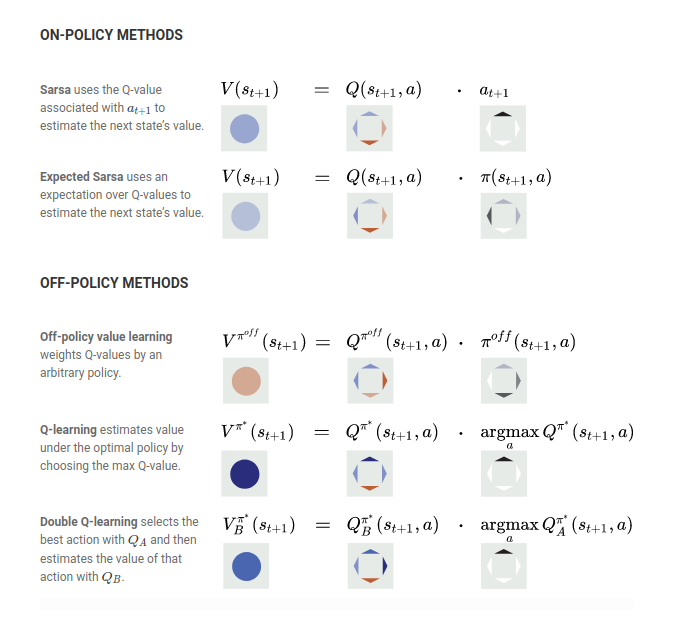
\includegraphics[width=500px]{../pics/td_methods.png}
	
\subsubsection{Learning by Cheating}

\begin{verbatim}
	https://arxiv.org/abs/1912.12294
\end{verbatim}

\begin{remark}
	Decompose imitation learning into two stages. First train cheating model copying expert and accessing ground state and then train sensorimotor model copying cheater
\end{remark}

\begin{remark}
	Advantages:
	\begin{enumerate}
		\item Privileged agent operates on compact space representation
		\item The priveleged agent provides stronger supervision
		\item Internal state of privileged agent "white box" ie. can be examined at will
	\end{enumerate}
\end{remark}

\subsubsection{A tutorial on bayesian optimization}

\begin{verbatim}
	https://arxiv.org/pdf/1012.2599.pdf
\end{verbatim}

\begin{remark}
	Value iteration(and q iteration) independent of policy.
\end{remark}

\begin{remark}
	Policy iteration vs. value iteration. Policy iteration faster under certain conditions. Simply becuase actions change less often. But hard to tell when we've converged.

	Value iteration gives us more info. 

	Note we still compute value function with policy iteration.

	Value iteration converges when we have no change. Policy iteration converges when at every we take the maximal action. 

	These only useful when we have full knowlege of the dynamics
\end{remark}

\begin{remark}
	TD/MC useful when we don't know the dynamics.
\end{remark}


\section{3/14}

\subsection{Goals}

\begin{enumerate}
	\item Finish complex
	\item Thesis
	\item Review complex
	\item Transcription
\end{enumerate}

\subsection{Complex Review}

\subsubsection{Fourier Stuff}

\begin{theorem}
	Phragmen-Lindelof Lemma: bounds F in a sector if bounded on boundary and sub-exponential
\end{theorem}

\begin{proof}
	$F_{\epsilon}(z) = F(z)e^{-\epsilon z^{3/2}}$. By construction $cos(3\theta /2)$ positive so we get good decay for $F_{\epsilon}$. Then if $|F_{\epsilon}| \leq 1$ then $|F| \leq 1$ via continuity.

	Let $M = sup|F_{\epsilon}|$ then $\exists w_j \to w$ toward M. It must be $w \in \partial S$ which is bounded by 1. So done. Key is that $w_j$ are bounded since $F_{\epsilon} \to 0$ as $|z| \to \infty$. 
\end{proof}

\begin{theorem}
	If $f \in \mathcal{F}_a$ then $|\hat{f}(\xi)| \leq B_f e^{-2\pib |\xi|}$ for $0 \leq b < a$
\end{theorem}

\begin{proof}
	If $b=0$
	\begin{align*}
		\hat{f}(\xi) = \int_{\R}f(x)e^{-2\pi i x \xi}dx \implies |\hat{f}(\xi)| \leq \int_{\R}|f(x)|dx \leq \int_{\R}\frac{A_f}{1+x^2}dx = \pi A_f
	\end{align*}
	If $b > 0$ the idea is to shift contour of integration down imaginary line. Note vertical sides go to 0 as $R \to \infty$ since norm is large. So can shift down with a negation.
\end{proof}

\begin{theorem}Fourier Inversion:

	$f(x) = \int_{\mathbb{R}} \hat{f}(\xi) e^{2\pi i x \xi}dx$
\end{theorem}

\begin{proof}
	First note when $A > 0$ and B real
	\begin{align*}
		\int_0^{\infty} e^{-(A+iB)\xi}d\xi = \frac{1}{A+iB}
	\end{align*}
	Via checking the finite case and sending to $\infty$. 

	Then we argue by splitting across im line. In the positive case we can simply use definition and interchange integration and resolve with cauchy's integral formula. For the other case we consider a reverse contour and apply the current result.
\end{proof}
	
\begin{theorem}
	If $f \in \mathcal{F}$ then
	\begin{align*}
		\sum_{n \in \Z} f(n) = \sum_{n \in \Z} \hat{f}(n)
	\end{align*}	
\end{theorem}

\begin{proof}
	Key Idea 1: Idea is to pick out points being summed as residues. First note $\frac{1}{e^{2\pi i z}-1}$ has simple poles with residue $1/2\pi i $ at integers. Then Apply residue formula to $\frac{f(z)}{e^{2\pi i z}-1}$ which generates residues with $\frac{f(n)}{2\pi i}$. Integrating over rectangle contour(off integers). 

	Key idea 2: We then CLEVERLY rewrite $\frac{1}{e^{2\pi i z}-1} = -\sum e^{2\pi i n z}$ if $|z| < 1$ and similarly for complement case. Allows us to rewrite as fourier transform 
\end{proof}

\begin{remark}Residue Formula Computation Tools:

Idea is to find contour s.t.
\begin{align*}
	\lim_{R \to \infty} \int_{\gamma_R} f(z)dz = \int_{-\infty}^{\infty}f(x)dx
\end{align*}

Which is easier to evaluate because we simply compute residues

\textbf{EX 1:}

Consider
\begin{align*}
	\int_{-\infty}^{\infty}\frac{dx}{1+x^2} = \pi 
\end{align*}

Using the half circle $\gamma_R$ we have
\begin{align*}
	\int_{\R}\frac{1}{1+x^2}dx = -\lim \int_{\gamma_R}\frac{1}{1+z^2}dz = -\lim \int_{\gamma_R}\frac{1}{(z-i)(z+i)}dz = 
\end{align*}

Partial fraction decomposion yields $\frac{1}{(z-i)(z+i)} = \frac{1}{2i}\frac{1}{z-i} - \frac{1}{2i}\frac{1}{z+i}$ so integrating over half ciricle gives $2\pi i/2 i = \pi$. 

Further note we have equality since the integral over the polar section goes to 0(b/c of large norm). 

\textbf{EX 2:}

Compute
\begin{align*}
	\int_{-\infty}^{\infty}\frac{e^{ax}}{1+e^x}dx
\end{align*}
For $0 < a < 1$

Consider the rectangle contour with height $2 \pi i$. Note $\pi i$ is a residue. To compute it we simply note

\begin{align*}
	\lim_{z \to \pi i} \frac{e^z - e^{\pi i}}{z - \pi i} = e^{\pi i} = -1
\end{align*}

showing it to be a simple pole(since we do not have blowup). 

\begin{align*}
	\int_{\gamma_R}\frac{e^{az}}{1+e^z}dz  = - 2\pi i e^{a \pi i} 
\end{align*}

Notice the vertical strips go to 0(Since $a < 1$) and we are done. 

\textbf{Ex 3:}

\begin{align*}
	\int_{\R} \frac{e^{-2\pi i x \xi}}{cosh(\pi x)}dx = \frac{1}{cosh(\pi \xi)}
\end{align*}

Sticking point: algebraically recognize
\begin{align*}
	e^{-2\pi i z \xi} \frac{2(z-\alpha)}{e^{\pi z}+e^{-\pi z}} = 2e^{-2\pi i z \xi} e^{\pi z}\frac{2(z-\alpha)}{e^{2\pi z}+e^{-\pi \alpha}}
\end{align*}

where right hand side difference quotient of $e^{2\pi z}$ ie. derivative. Which we can compute

Key Theme: Recognizing difference quotients and using them to compute
	
\end{remark}

\begin{theorem}
	Riemann theorem on removable singularities:
\end{theorem}

\begin{proof}
	Key idea is to extend $f$ to $z_0$ with cauchy's formula. It suffices to show $f(z) = \int_C \frac{f(\xi)}{\xi -z} d\xi$. 

	Using a double keyhole we evaluate the integral to see $\int_C \frac{f(\xi)}{\xi - z}d\xi + \int_{\gamma_{z_0}} \frac{f(\xi)}{\xi - z}d \xi + \int_{\gamma_{z}} \frac{f(\xi)}{\xi - z}d \xi = 0$. We know cauchy formula holds at $z$ and is small over $\gamma_{z_0}$ since boundedness and small $\epsilon$ circle. THIS IS WHERE WE USE BOUNDEDNESS, to control small circles around $z_0$

	Remark:

	1. Boundedness use to control small circles around $z_0$

	2. Holomorphicity used for cauchy formula
\end{proof}

\begin{theorem}
	Casorate-Weierstrass: f holomorphic. If $z_0$ not a removable discontinuity then the image dense in $\C$. 
\end{theorem}

\begin{proof}
	We go by contradiction. Suppose not dense. To some $w \in \C$. Then consider $g(z) = \frac{1}{f(z) - w}$. Is bounded. Hence $g(z_0)$ removable singularity at $z_0$. If $g(z_0) \neq 0$ then $f(z) - w$ holomorphic at $z_0$ a contradiciont. Otherwise is a pole, again a contradiction. 

	Key idea: Look at function combining w and f and examining singularities. 
\end{proof}

\begin{theorem}
	Meromorphic functions in extended complex plane are rational
\end{theorem}

\begin{proof}
	Decompose $f = f_k + g_k$ into principle and holomorphic parts at singularity $z_k$. Idea is to subtract off principal parts and principal reciprocal parts and show remainder constant. 
\end{proof}

\begin{quest}
	Why does this suffice to show rational?
\end{quest}

\begin{theorem}
	Argument Principle: Num zeroes - num poles = $\frac{1}{2 \pi i}\int_{D_R} \frac{f'}{f}$
\end{theorem}

\begin{proof}
	The key is $f'/f = n/z-z_0 + g(z)$ at a zero where g holomorphic. Similar formula but minus for a singularity. 
\end{proof}

\begin{theorem}
	Rouche: If $|f| \geq |g|$ both holo then $f$ and $f+g$ have same number of 0s in $\Omega$. 
\end{theorem}

\begin{proof}
	We go by the argument principle. Both holo so $1/2\pi i \int_C f'/f$ counts zeroes. 

	We define $h_t(z) = tf(z) +(1-t)g(z)$. 
\end{proof}

\section{3/15}

\subsection{Goals}

\begin{enumerate}
	\item exam
	\item work on thesis/research
	\item Transcription
	\item complex homework
	\item Bonus: Grind DRL
\end{enumerate}

\subsection{Questions}

\begin{remark}
Complex:
\begin{enumerate}
	\item 1 on complex exam
	\item 2 on complex exam
	\item Hw 5.1 how do we have continuity of f? DCT?
\end{enumerate}
\end{remark}

\begin{remark}
Jazz:
\begin{enumerate}
	\item Measure 14 upbeat of 3 what notes?
	\item How to distinguish more than one note?
	\item What is this rhythm at measure 17? - Trills
\end{enumerate}
\end{remark}

\subsection{DRL}

\begin{remark}
	Gaussian process resource:
	\begin{verbatim}
		http://mlg.eng.cam.ac.uk/teaching/4f13/1920/gp%20and%20data.pdf
	\end{verbatim}
\end{remark}

\section{3/16}

\subsection{Goals}

\begin{enumerate}
	\item Go to open house
	\item Revamp site/apply to summer stuff
	\item Finish DRL
	\item Work on thesis
	\item start complex
\end{enumerate}

\subsection{DRL}

\begin{remark}
	MCTS: Keeps tree of nodes that is slowly expanded and which we keep q-values for. All concentrated on one state
\end{remark}

\begin{remark}
	MCTS does not form q values for nodes in random phase.
\end{remark}

\begin{quest}
	Is model free method like DQN more or less accurate than MCTS.
\end{quest}

\begin{ans}
	MCTS since concentrated on one state. But slow
\end{ans}

\subsection{Deep Learning for Real-Time Atari Game Play Using Offline Monte-Carlo Tree Search Planning}

\begin{verbatim}
	https://papers.nips.cc/paper/2014/hash/8bb88f80d334b1869781beb89f7b73be-Abstract.html
\end{verbatim}

\subsection{Playing Atari with Deep Reinforcement Learning}

\begin{verbatim}
	https://arxiv.org/pdf/1312.5602.pdf
\end{verbatim}

\subsection{Modeling Evolution}

\subsection{DRL}

\section{3/17}

\subsection{Goals}

\begin{enumerate}
	\item Finish chapter of thesis
	\item Finish DRL
	\item Start complex
	\item summer thing
\end{enumerate}

\subsection{Questions}

\begin{remark}
	DRL:
	\begin{enumerate}
		\item How is regret defined in bandit lecture? What is optimal policy here?
	\end{enumeate}
\end{remark}

\section{3/18}

\subsection{Goals}

\begin{enumerate}
	\item Finish chapter of thesis
	\item Finish DRL
	\item Rough out complex
	\item Grind transcription
\end{enumerate}


\end{document}

